%!TEX root=../GaugeCNNTheory.tex


\subsection{Coordinate independent feature vector fields}
\label{sec:feature_fields}

The feature spaces of coordinate independent CNNs are spaces of feature vector fields.
Similar to the case of tangent vectors coefficients, the numerical coefficients of feature vectors are required to transform consistently under gauge transformations.
The specific transformation law (group representation) of a feature field does hereby specify its field type -- common examples are scalar fields, tangent vector fields, general tensor fields, regular feature fields or irrep fields.
Section~\ref{sec:individual_fields} introduces such feature fields and their transformation laws.
In Section~\ref{sec:stacked_fields}, we briefly define coordinate independent feature spaces.
Similar to the definition of the feature spaces of conventional CNNs as stacks of multiple feature maps, the feature spaces of coordinate independent CNNs consist of multiple independent feature fields.




\subsubsection{Individual feature vector fields}
\label{sec:individual_fields}
Convolutional feature fields assign a feature vector, encoding information inferred from a local neighborhood of the input signal, to each point of the manifold.
The spatial accumulation of information is performed by a convolutional kernel which is \emph{measuring feature fields} in its surrounding \emph{relative to its local reference frame}.
We are thus assuming a gauge $\psi^A$ which specifies the kernel alignments on a neighborhood $U^A$.
Relative to this gauge the kernel will yield a smooth local field of responses (observations)
\begin{align}
    f^A:U^A\to\R^c \,,
\end{align}
given by a $c$-dimensional numerical feature vector $f^A(p)$ at each position $p\in U^A$.
Assume a second response field $f^B:U^B\to\R^c$, inferred relative to gauge $\psi^B$ on $U^B$, to be given.
Since the response of a kernel depends in general on its alignment, it is to be expected that $f^A$ and $f^B$ do not agree on the overlap $U^A\cap U^B.$
Without further restrictions the responses of a convolution kernel will be arbitrarily gauge dependent.

\begin{figure}
    \centering
    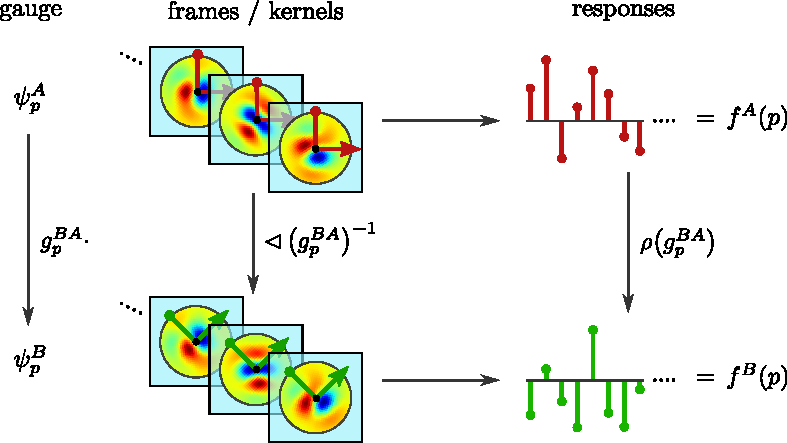
\includegraphics[width=.75\columnwidth]{figures/kernel_responses.pdf}
    \vspace*{1ex}
    \caption{\small
        The numerical responses $f^A(p) \in\R^c$ and $f^B(p) \in\R^c$ of kernels that are oriented according to different frames do in general not coincide.
        In order to represent numerical coefficients of the \emph{same coordinate independent feature vector} relative to the chosen gauge, they are required to be related by gauge transformations $\rho(g_p^{BA})$ if the gauges are related by~$g_p^{BA}$.
        As derived in Section~\ref{sec:gauge_CNNs_local}, this requirement imposes a gauge equivariance constraint on the convolution kernels.
        }
    \label{fig:gauge_trafos_feature_vector}
\end{figure}

\begin{minipage}{\textwidth}
The \emph{principle of covariance}, proposed by Albert Einstein \cite{Einstein1916German,Einstein1916English}, states that:
\vspace*{1.ex}
\begin{center}
    \it
    ``Universal laws of nature are to be expressed by equations which hold good for all systems
    \\
    of coordinates, that is, are covariant with respect to any substitutions whatever.''
\end{center}
\vspace*{1.ex}
\end{minipage}
We believe that a similar principle should hold in geometric deep learning as well, that is, the inference should be independent from any arbitrariness in the choice of reference frames.
Given that this arbitrariness in coordinatizations is precisely captured by the given $G$-structure $\GM$, this requires in particular that \emph{features should be $\GM$-coordinate independent} geometric objects.%
\footnote{
    In this point we deviate from Einstein's \emph{general} covariance, which always considers $\GL{d}$-valued gauge transformations (corresponding to diffeomorphism covariance).
    His setting is in our formulation included for $G=\GL{d}$, however, we keep the assumed structure group flexible since most applications will assume a reduced structure group.
}
We thus design convolution kernels such that their responses $f^A$ and $f^B$ encode fields of \emph{feature vector coefficients} which \emph{represent a coordinate free feature vector field $f$} locally in different gauges.
A collection of such numerical coefficient fields $f^X$, expressed relative to a $G$-atlas of gauges $\psi^X$ on neighborhoods $U^X$ covering $M$, is equivalent to the global, coordinate free feature field $f$ on~$M$.


\begin{figure}
    \centering
    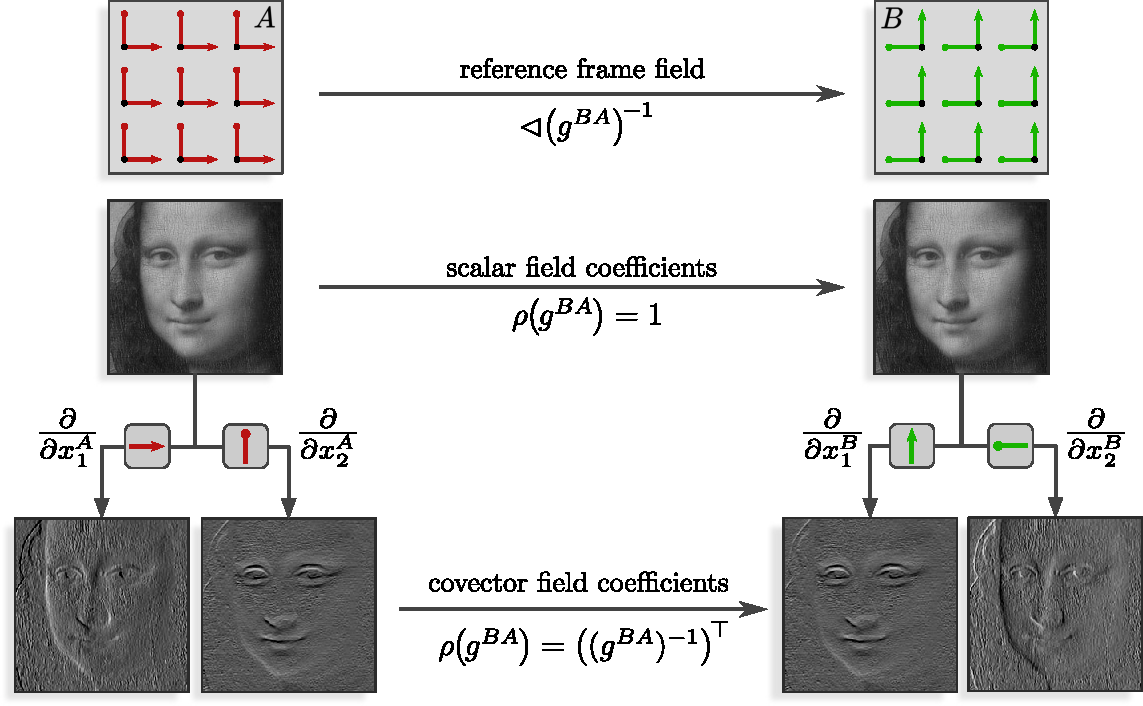
\includegraphics[width=.83\columnwidth]{figures/mona_lisa_gradient.pdf}
    \caption{\small
        Examples of feature coefficient fields on $M=\R^2$ from classical image processing.
        \ \emph{Top}:
        For simplicity we assume a ``parallel'' frame field and consider the same gauge transformation, a rotation by $\pi/2$, at each point $p\in M$.
        \ \emph{Middle}:
        The intensity values of a grayscale image are independent from the choice of reference frames.
        They are therefore modeled by scalar fields, characterized by the trivial representation $\rho(g)=1\ \forall g\in G$.
        \ \emph{Bottom}:
        The two coefficient channels of a gradient image are calculated from a scalar image by taking the derivatives along the frame axes -- they are therefore gauge dependent.
        Gradient images w.r.t. different gauges are related by the group representation $\rho(g)=(g^{-1})^\top$ and are therefore identified as covector fields (tensor fields of type $(0,1)$ or 1-forms).
        For~the visualized rotation by $\pi/2$ this leads to a new first channel $(\nicefrac{\partial}{\partial x_1^B})$ equivalent to the old second channel $(\nicefrac{\partial}{\partial x_2^A})$ and a new second channel $(\nicefrac{\partial}{\partial x_2^B})$ equivalent to the negative old first channel $(\nicefrac{\partial}{\partial x_1^A})$.
        Relative to their respective reference frames, both coefficient fields encode the same (coordinate free) gradient field.
        The description is therefore automatically coordinate independent.
    }
    \label{fig:feature_field_gradient}
\end{figure}

In order for this coordinate free feature field to be well defined, i.e. $\GM$-coordinate independent, the local coefficient fields (or kernel responses) are required to be consistently stitched together via $G$-valued transition maps.
They must therefore transform in a principled manner under gauge transformations.
Since we are dealing with feature vector spaces, these transformations are typically taken to be linear, that is, they are modeled by linear \emph{group representations}
\begin{align}\label{eq:group_representation}
    \rho:G\to\GL{c}
\end{align}
of the structure group $G\leq\GL{c}$, which operates on $\R^c$ and satisfies $\rho(gh)=\rho(g)\rho(h)\ \forall\ g,h\in G$.%
\footnote{\label{footnote:repr_group_homomorphism}
    This condition ensures that representations are group homomorphisms, i.e. maps which respect the group structure of~$G$.
    The actions of the structure group on the tangent space and feature vector coefficient spaces are thus compatible.
}
Similar to the transformation of tangent vector coefficients in Eq.~\eqref{eq:components_leftaction}, the feature vector coefficients are then defined to transform under a $G$-valued gauge transformation $g_p^{BA}=\psi_p^B\!\circ\!\left(\psi_p^A\right)^{-1}$ like
\begin{align}\label{eq:gauge_trafo_features}
  f^B(p)\ :=\ \rho\big( g_p^{BA}\big) f^A(p) \,,
\end{align}
where $p\in U^A\cap U^B$; see Fig.~\ref{fig:gauge_trafos_feature_vector} for a visualization.
Being constructed to transform synchronously, the spaces of reference frames, tangent vector coefficients and feature vector coefficients are said to be $G$-\emph{associated} to each other.
Note that the construction via a $G$-representation $\rho$ does in general \emph{not} describe $\GL{d}$-valued gauge transformations, i.e. fully coordinate independent features.
The extracted feature vectors will therefore only have a well defined expression relative to the frames in the considered $G$-structure $\GM$, which is captured by the term ``$\GM$-coordinate independence''.


Different choices of representations $\rho_i$ yield different \emph{types} of feature fields as exemplified in Fig.~\ref{fig:feature_field_gradient}.
For instance, the trivial representation, $\rho(g)=1\ \forall g\in G$, describes the transformation behavior of \emph{scalar fields} $s^A(p)\ \mapsto\ s^B(p)\ :=\ 1\cdot s^A(p)$, whose numerical coefficients are invariant under gauge transformations.
Example of scalar fields are grayscale images, temperature fields, pressure fields or probability distributions on $M$.
The coefficients of \emph{tangent vector fields} transform like $v^A(p)\ \mapsto\ v^B(p)\ :=\ g_p^{BA}v^A(p)$ and correspond therefore to the group representation $\rho(g)=g$.
Examples for vector fields include optical flow or wind velocity fields.
More general tensor fields of type $(r,s)$ are described by tensor product representations $\rho(g) = \otimes^s\left(g^{-1}\right)^{\!\top} \otimes^r g$.
They model for instance diffusion tensor images, electromagnetic field tensors or stress tensors.
A common choice for discrete structure groups are \emph{regular representations} which realize the finite set of group operations by permutation matrices.
Regular representations arise as exact symmetries of crystal lattices, spin lattices or pixel grids~\cite{Cohen2016-GCNN,Hoogeboom2018-HEX,winkels3DGCNNsPulmonary2018,Worrall2018-CUBENET,gaugeIco2019}.
In addition, they are commonly used as discrete approximation of continuous structure groups, e.g. cyclic groups $C_N\leq\SO2$ to approximate continuous rotations~\cite{Weiler2018SFCNN,bekkers2018roto,Weiler2019_E2CNN,bekkers2020bspline,Marcos2017-VFN}.
They are of great practical relevance since they describe the transformation of the features of group convolutional networks~\cite{Cohen2016-GCNN}.
Feature fields which transform under \emph{irreducible representations} (irreps) were investigated in~\cite{Worrall2017-HNET,3d_steerableCNNs,Thomas2018-TFN,Kondor2018-NBN,anderson2019cormorant,Weiler2019_E2CNN,jiang2019spherical}.%
\footnote{
\label{footnote:feature_field_irrep_decomposition}
    By the Peter-Weyl Theorem, any unitary representation of a compact group can via a change of basis be decomposed into a direct sum of irreps.
    This implies that any \emph{linear} neural network operation between general representations can (after a change of basis) be understood in terms of operations between irreps~\cite{Weiler2019_E2CNN,lang2020WignerEckart}.
    In contrast, the specific choice of representation, i.e. the change of basis relative to the irreps contained in it, \emph{does} matter for any \emph{non-linear} network layer.
}
A more detailed overview and an extensive benchmark of different field types or representations in deep learning was presented in~\cite{Weiler2019_E2CNN}.


For completeness we want to mention that coordinate free feature vector fields are formally defined as smooth sections $f\in\Gamma(\A)$ of a \emph{feature vector bundle} $\A\piAarrow M$ which is associated to the $G$-structure $\GM$ and has the feature vector coefficient spaces $\R^c$ as typical fibers.
The coefficient vectors $f^A(p)$ and $f^B(p)$ in $\R^c$ are local trivializations of a coordinate free feature vector $f(p) \in \A_p \cong \R^c$, and are similarly defined as the coefficients $v^A=\psi_p^A(v)$ and $v^B=\psi_p^B(v)$ of a tangent vector $v\in \TpM$.
Note that, while being isomorphic, the feature spaces $\A_p \cong \A_q$ at different points $p\neq q$ of~$M$ are distinct from each other, such that their elements can not be summed together.
The parallel transporters, discussed in Sections~\ref{sec:transport_local} and~\ref{sec:bundle_transport}, provide isomorphisms between different feature vector spaces, which allows the summation of features (after transporting them into the same vector space).
Since these definitions are quite technical, we skip their details for now and refer the interested reader to Section~\ref{sec:G_associated_bundles}.








\subsubsection{Stacked feature fields and coordinate independent feature spaces}
\label{sec:stacked_fields}

\begin{wrapfigure}[12]{r}{0.365\textwidth}
    \vspace*{-4.25ex}
    \hfill
    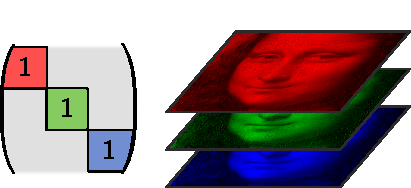
\includegraphics[width=.95\linewidth]{figures/feature_field_RGB.pdf}%
    \vspace*{.0ex}
    \captionsetup{width=.35\textwidth}
    \caption{\small
        The three color channels of an RGB image are identified as scalar fields, the full feature space therefore transforms according to $\rho(g) = (\mkern1.5mu 1 \mkern1.5mu) \oplus (\mkern1.5mu 1 \mkern1.5mu) \oplus (\mkern1.5mu 1 \mkern1.5mu)$.
        }
    \label{fig:feature_space_RGB}
\end{wrapfigure}%
The feature spaces of conventional CNNs consist of multiple feature maps.
In analogy, we define the feature spaces of coordinate independent CNNs to comprise multiple feature fields $f_i$ of potentially different types $\rho_i$ and dimensionalities $c_i$.
A full field of activations of a feature space of a coordinate independent CNN is therefore defined as the \emph{direct sum}%
\footnote{
    The direct sum $\oplus$ of vectors $f_i(p)$ can be thought of as ``stacking'' these into a concatenated vector.
    Consistently with this, the direct sum of representations $\rho_i$ can be thought of as building a block diagonal matrix containing the $\rho_i$ as blocks; see Figs.~\ref{fig:feature_space_RGB} and~\ref{fig:feature_spaces_oplus}.
}
\begin{align}\label{eq:feature_field_full}
    f = \scalebox{1.1}{$\bigoplus$}_i f_i
\end{align}
of the individual fields.
Every feature map of a conventional CNN encodes the position of a particular feature and transforms independently when the network's input is shifted.
The individual feature fields $f_i$ of $\GM$-coordinate independent CNNs encode both the position and the $G$-pose of a feature.
In contrast to conventional feature maps, their coefficient fields, for instance $f_i^A$, are additionally guaranteed to transform independently from each other under gauge transformations as specified by their type ${\rho_i:G\to\GL{{c_i}}}$.
A~local numerical representation $f^A = \bigoplus_i f_i^A$ of the full feature field in Eq.~\eqref{eq:feature_field_full} transforms therefore according to the direct sum of the individual representations, that is,
\begin{align}
    \rho = \scalebox{1.1}{$\bigoplus$}_i \rho_i \,.
\end{align}
The independent transformation of individual fields under $\rho$, visualized in Fig.~\ref{fig:feature_spaces_oplus}, is clear by construction:
\begin{align}
    \rho(g)f^A
    \,=\, \left(\scalebox{1.1}{$\bigoplus$}_i \rho_i(g)\right) \! \left(\scalebox{1.1}{$\bigoplus$}_i f_i^A\right)
    \,=\, \scalebox{1.1}{$\bigoplus$}_i \! \left(\rho_i(g) f_i^A\right)
\end{align}

\begin{figure}
    \centering
    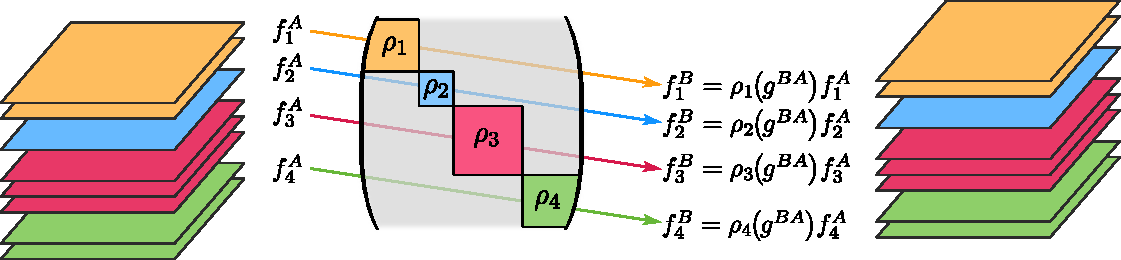
\includegraphics[width=.94\textwidth]{figures/feature_field_repr_examples.pdf}
    \vspace*{0ex}
    \caption{\small
        A full feature space comprises multiple individual feature fields $f_i$ of potentially different types $\rho_i$ and dimensionalities $c_i$.
        Via a gauge $\psi^A$, it is locally represented by coefficient fields $f_i^A: U^A \to \R^{c_i}$.
        The coefficient fields in another gauge $\psi_B$ are related via a gauge transformation $f_i^B = \rho_i\big(g^{BA}\big)f_i^A$.
        The coefficients of each individual field transform independently, the representation modeling the whole feature space is thus given by the direct sum, here $\bigoplus_i \!\rho_i = \rho_1 \oplus \rho_2 \oplus \rho_3 \oplus \rho_4$.
    }
    \label{fig:feature_spaces_oplus}
\end{figure}

As a practical example of a coordinate independent feature space consisting of multiple fields consider an RGB image as depicted in Fig.~\ref{fig:feature_space_RGB}.
Like the grayscale image in Fig.~\ref{fig:feature_field_gradient}, the individual color channels encode intensity values which are invariant under gauge transformations.
The full RGB image is therefore to be identified with three scalar fields, each of which ``transforms'' independently under the trivial representation.
Not all individual feature fields need to be of the same type $\rho_i$.
For instance, in a weather forecasting application the input signal might consist of scalar fields encoding features like temperature or pressure and vector fields like wind speeds.
A description as $\rho_i$ fields of corresponding types ensures the geometrically correct processing of such data.
While the field types $\rho_i$ of a network's input and output are typically given by the learning task, the field types used in hidden layers are chosen by the user as a hyperparameter similar to the choice of channels for a conventional CNN.